\chapter{Product Concept}
\setlength{\headheight}{22.94003pt}
\addtolength{\topmargin}{-10.22661pt}

It is estimated that only 35\% of the globally produced plant protein is consumed by humans. Meanwhile the current market offers a wide range of plant-based proteins available which are well fitted for human consumption. Common choices include formulations with oat, wheat, hemp, soy and pea to name a few (Gorissen et al., 2018). The Cannabis sativa L., a Cannabaceae known as ‘‘hemp’’ is of increasing interest because it is highlighted as an environmentally friendly and economically high-potential crop. Its history as a source for medicine, fiber and food dates back 6000 years, and the cultivation of hemp with close to no levels of tetrahydrocannabinol (THC), the psychoactive compound found in cannabis, has increased to use in foods since strains with a THC content below 0.3\% was approved in EU in 1996. Among its many advantages are fast growth and low dependency on pesticides, which benefits biodiversity and healthy soils. Furthermore, its seeds provide a valuable source of nutrients. (Chapter 6 Industrial Hemp Seed). Globally, the trend of increasing interest for hemp seeds is clear, as the production increased from 2,718 tons to 5,449 tons between 2015 and 2020. 

\vspace{1em}
Thus, developing a convenient hemp-based bar would harness the many benefits of the not-so-novel ingredient that is hemp seed. Below is a mock up of the Hemp Protein Bar (figure 4).

\begin{figure}[H]
    \centering
    \includegraphics[width=0.54\linewidth]{Figures/fig_prod_concept_01.png}
    \caption{AI-generated illustration of a medieval marketplace. Generated using DALL·E 3 (OpenAI, 2025) with the prompt: "Mock up of a hemp bar picture half coved in chocolate ".}
    \label{fig:prod_concept_01}
\end{figure}


\section{Macronutrients in Hemp Seeds}
Hemp seeds typically contain around 20-30\% protein, 25\%-35\% lipids, 20-30\% carbohydrates and 4-7\% of ash (Figure 5). It has a balanced composition with particularly low starch content. (Montero et al 2023) 

\begin{figure}[H]
    \centering
    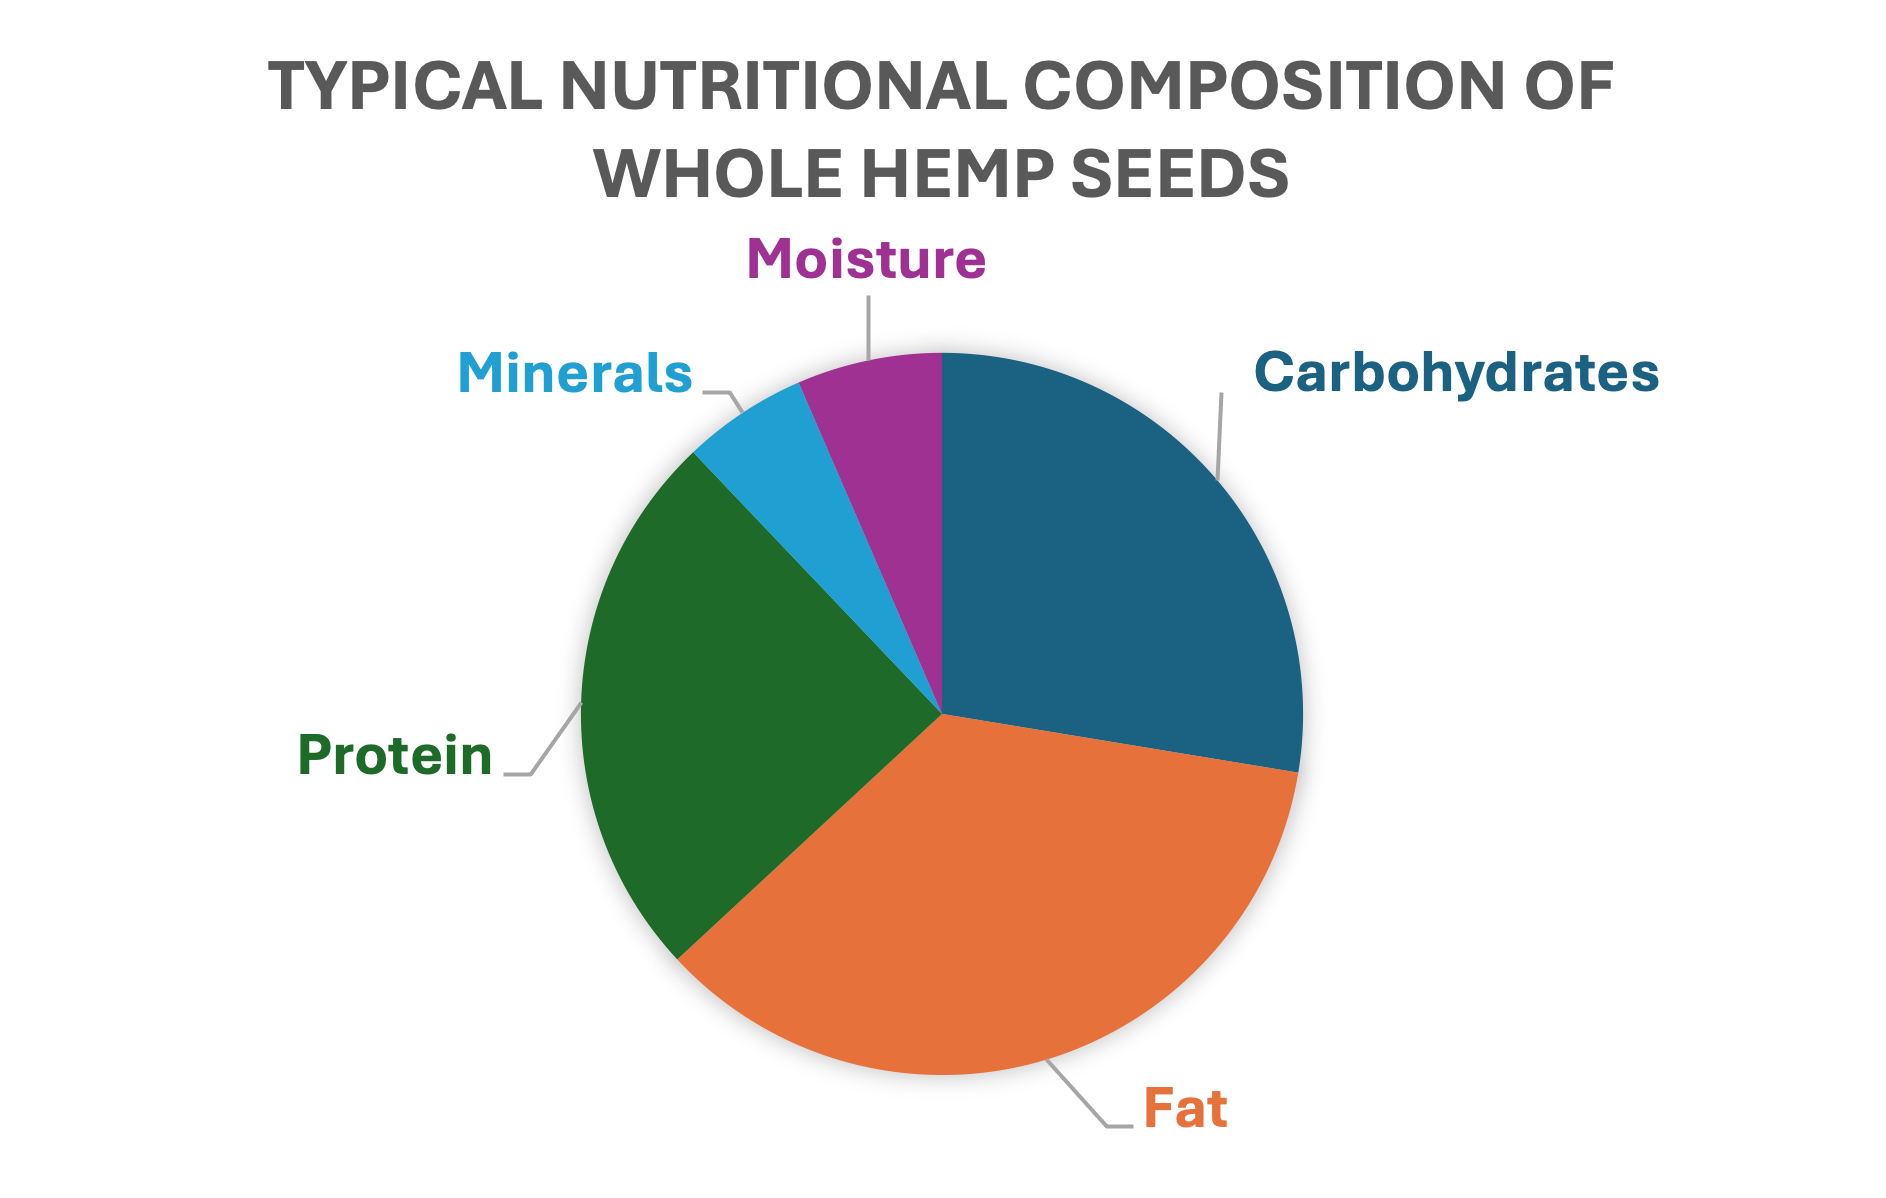
\includegraphics[width=0.75\linewidth]{Figures/fig_prod_concept_02.png}
    \caption{Composition diagram of whole hemp seeds}
    \label{fig:prod_concept_02}
\end{figure}

\subsection{Protein}
Hemp seeds are an excellent source of high-quality protein, typically containing 20–30\% protein, with dehulled hemp seeds having even higher protein contents, ranging from 30\% to 38\%. (chapter 4 hemp seed book). The two main proteins in hemp seeds are albumin (33\%) and edistin (65\%), which have very similar structures to plasma proteins which helps the digestibility in humans. Hemp seeds provide a complete amino acid profile, containing all nine essential amino acids required by humans, making them comparable to other high-quality proteins like egg white and soybeans (Chapter 10). 

\vspace{1em}
The protein is also particularly rich in arginine, glutamic acid, and aspartic acid, where arginine is especially valuable as it is a precursor to nitric oxide, which enhances blood flow and helps maintain normal blood pressure, contributing to cardiovascular health (chapter 11 hemp book)
Hemp proteins are highly digestible, with dehulled hemp seeds demonstrating superior protein digestibility (83.5–92.1\%) (hemp nutritional value). This is partly attributed to the absence of protease inhibitors in hemp seeds (Hemp seed bioactivity). 

\vspace{1em}
A study has analysed the macronutrient composition and protein quality of 30 hemp seed products from Western Canada, including whole seeds, dehulled seeds, and hemp seed meal. Crude protein, fat, and amino acid profiles were determined, and protein quality was assessed using the Protein Digestibility-Corrected Amino Acid Score (PDCAAS) method, based on a rat bioassay and FAO/WHO amino acid requirements for young children. Average protein content ranged from 24.0\% in whole seeds to 40.7\% in hemp seed meal. Protein digestibility was 84–98\%, with protein digestibility-corrected amino acid score (PDCAAS) values of 46–66\%, highest in dehulled seeds. The protein digestibility-corrected amino acid score of dehulled hemp seed is comparable to lentils and is about half that of casein, and almost twice that of almonds (chapter 10 hemp seed book)

\subsection{Fatty Acids}
Hemp seed oil is primarily composed of polyunsaturated fatty acids, PUFA (over 80\%) including fatty acids like essential linoleic acid (omega-6) and alpha-linolenic acid (omega-3). (Chapter 10 hemp seed book) Dehulled hempseeds have a healthy balance of omega-6 to omega-3 polyunsaturated fatty acids (2.5:1) (Chapter 1 hemp book)

\vspace{1em}
Unsaturated fatty acids help protect against cardiovascular disease, obesity, diabetes, and inflammation. EFSA recommends an optimal omega-6/omega-3 ratio of 3:1 to 5:1. Hemp seed oil typically shows a ratio of 2.5–3.5:1, which is a desirable range linked to lower chronic disease risk. (Hemp nutritional value pdf)

\section{Carbohydrates}
About 98\% of the carbohydrates in hemp seeds are dietary fiber, mainly insoluble dietary fibers (80\%), such as cellulose, lignin and hemicellulose. Dietary fiber resists enzymatic digestion in the small intestine and undergoes partial or complete fermentation in the large intestine. The remainder of the carbohydrates in hemp seeds is starch. Therefore, hemp seeds are considered a low-starch food and an excellent source of dietary fiber. (Hemp nutritional value pdf) 

\vspace{1em}
The dietary fibers from hemp seeds are associated with positive effects on the digestive tract support by acting as prebiotics. The fermentation of fibers in the colon generates short-chain fatty acids that have beneficial roles in the body. (Hemp seed bioactivity pdf). In the Western countries the consumption of dietary fiber is lower than the recommended intake, making hemp seeds an attractive ingredient to meet the recommended daily intake of dietary. However, processing might affect the amounts of dietary fibers in hemp seeds. 

\section{Micronutrients: Vitamins and Minerals}
Hemp seeds are rich in vitamins and minerals. Just 50 mg of hemp seed can supply at least half of the recommended daily allowance of copper, magnesium, and zinc, and exceed the recommended daily allowance of the vitamins A, D, and E. (Chapter 1 hemp book) Hemp seeds also contain other micronutrients such as phosphorus, potassium, calcium, sodium, iron, and manganese. (Chapter 4 hemp book). Hemp seed oil contains fat-soluble vitamins, in particular vitamin E (tocopherols) and vitamin A which respectively has an antioxidant role and is beneficial for skin integrity and Vitamin D is important for bone health and the immune system (Hemp nutritional value pdf)

\vspace{1em}
Besides the macro- and micronutrients, secondary metabolites, such as terpenes, phytosterols and flavonoids, constitute essential components of the defence response of the hemp plant to biotic and abiotic stresses. However, the composition of these secondary metabolites can be influenced by cultivation conditions, providing a distinct fingerprint of different production regions. It is suggested that these compounds contribute with antioxidative, antimicrobial, and anti-inflammatory properties in the human body. Phytosterols for instance, are not synthesized in humans, but can when ingested from plants, reduce cholesterol levels in the human body by changing the cholesterol solubility in the intestine. (Tănase et al. 2024).

\section{Potential Side Streams}
The industrial hemp plant has a versatile plant body which consists of seeds, leaves, stem, and flowers with several application opportunities depending on the part of the plant. Particularly the stem is a valuable source to produce hemp fiber which can be used for rope, building materials, paper, or textiles. The seeds, dehulled or whole, can be utilized as a food source. The hemp flower can be used to produce cosmetic and pharmaceutical products, including essential oils. When looking further into hemp as a natural source to bast fiber a life cycle assessment reveals that hemp performs better than glass fiber by weight and compared to cotton, hemp requires less water and pesticides to grow although hemp fiber is known to be coarser and stiffer than cotton which has a softer appearance. (Kaur \& Kander 2023). 

\vspace{1em}
When processing the stem to hemp fiber a by-product of shives is made. It can be used to produce hemp concrete which is a bio-composite and carbon-negative alternative to concrete for construction and insulation. (Yano \& Fu 2023). These useful side streams make hemp even more attractive to use as an ingredient in foods. 

\section{Dietary Pattern of the Chosen Consumer Group and Product Fit}
Our hemp seed bar is uniquely positioned to seamlessly integrate into several contemporary dietary patterns, directly addressing the needs and preferences of our diverse target consumer groups within the Millennial and Generation Z age group.

\vspace{1em}
For vegetarians and vegans dehulled hemp seeds are an excellent source of high-quality, plant-based protein. The seeds naturally contain all nine essential amino acids required by humans, offering a complete protein profile that can be challenging to obtain from other plant sources. (Chapter 1 hemp seed book) The protein in dehulled hemp seeds also boasts superior digestibility (83.5\%-92.1\%) compared to whole hemp seeds and hemp meal, making its nutrients more accessible. They also provide a healthy balance of omega-6 to omega-3 polyunsaturated fatty acids (typically 2.5:1 to 3.5:1), which is desirable for overall human nutrition. (Hemp nutritional value pdf) Hemp protein and flour can serve as an alternative for soy ingredients (Chemical composition and biological activities of PDF) 

\vspace{1em}
A health-conscious person or athlete would also use it for its excellent source of protein, especially because of the high value protein composition with the nine essential amino acids. Furthermore, it scores high in terms of digestibility which makes our bar effective for muscle recovery and satiety. (Chapter 10 hemp book) Many athletes need to have control on their calorie needs. Our bar could therefore be an easy boost of calories or be used as a substitute for a snack or meal.
\vspace{0.5em}
The bar is rich in healthy fats, including the beneficial omega-6 to omega-3 ratio, which is important for cardiovascular health and may help prevent chronic diseases. (Hemp nutritional value pdf)

\vspace{1em}
Our bar is also a good source of essential minerals like copper, magnesium, and zinc, and provide vitamins A, D, and E, which also talks to the health-conscious person (Chapter 1 hemp book)

\vspace{1em}
For individuals with dietary restrictions and/or allergies our bar is also a great option, as our bar is naturally gluten-free, making it a safe nutritious option for people with celiac disease or gluten sensitivities. (Chapter 1 hemp book) Hemp proteins are generally considered to have low allergenicity compared to common proteins like soy, dairy, or wheat, broadening its appeal for those with various food allergies. (Chapter 11 hemp book \& Hemp nutritional value pdf)

\vspace{1em}
For environmentally aware consumers our hemp-based product directly supports environmental sustainability due to it having a low environmental impact, actively contributing to improved soil health, water quality, have carbon-negative crops and requiring no or little pesticide use. (Chapter 1 hemp book \& hemp nutritional value PDF \& hemp seed bioactivity) 

\vspace{1em}
The pre-packaged protein bar format offers convenience and time efficiency, requiring no preparation or cleanup for the people on-the-go. It delivers the balanced nutrition derived from dehulled hemp seeds in an easily consumable form, perfectly fitting the needs of busy individuals seeking healthy and convenient dietary options.


